\begin{figure}[ht]
    \centering
    \caption{Arquivo de texto simples, texto não formatado, aberto para edição no xed.}
    \begin{center}
        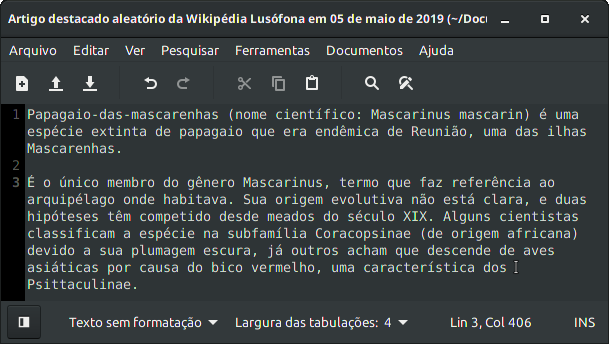
\includegraphics[width=0.75\textwidth]{img/exemplo-texto-simples.png}
    \end{center}
    \vspace{-0.5cm}
    \legend{\ABNTEXfontereduzida \textbf{Fonte:} O autor, conteúdo do texto obtido de \citeonline{Wikipedia_ConteudoDest05maio_2019}.}
    \label{fig:exemplo-texto-simples}
\end{figure}

